% Farbe fuer die Abbildung dieses Kapitels. Bewusst als abgestufte Blautoene
% gewaehlt, damit die Grafik auch im Schwarz-Weiss-Druck lesbar bleibt.
\definecolor{nakblue}{RGB}{0,0,89}

\section{Herausforderungen (Kettner)}
\label{sec:herausforderungen}

Den dargestellten Chancen stehen Herausforderungen gegenüber, die entsprechend der eingangs formulierten Position nicht als gleichwertige Gegenargumente, sondern als notwendige Bedingungen behandelt werden. Sie beschreiben, welche rechtlichen, technischen und gesellschaftlichen Voraussetzungen ein verantwortungsvoller Einsatz erfordert. Betrachtet werden dazu Datenschutz, \acs{IT}-Sicherheit, Abhängigkeit und Ethik.

\subsection{Datenschutz}
\label{subsec:datenschutz}

Der Datenschutz ergibt sich aus der in Abschnitt~\ref{subsec:cloud} beschriebenen Architektur: Das Aktivierungswort entscheidet, was das Gerät verlässt. Dieses Schutzkonzept ist jedoch nur so belastbar wie die Erkennung selbst. Eine Untersuchung von elf Smart Speakern acht Hersteller wies mehrere hundert Fehlauslösungen durch alltägliche Medieninhalte nach \cite{schoenherr2022accidental}. Zudem ist die Verarbeitung den Nutzenden häufig nicht bewusst. Von 116 Befragten kannten nur 44,0\,\% die Überprüfungsseite ihres Anbieters, lediglich 8\,\% hatten dort jemals eine Aufnahme gelöscht (Abbildung~\ref{fig:kontrolltrichter}) \cite{malkin2019privacy}. Die in Abschnitt~\ref{subsec:cloud} beschriebenen Kontrollen erreichen also kaum jemanden.

\begin{figure}[!htb]
	\centering
	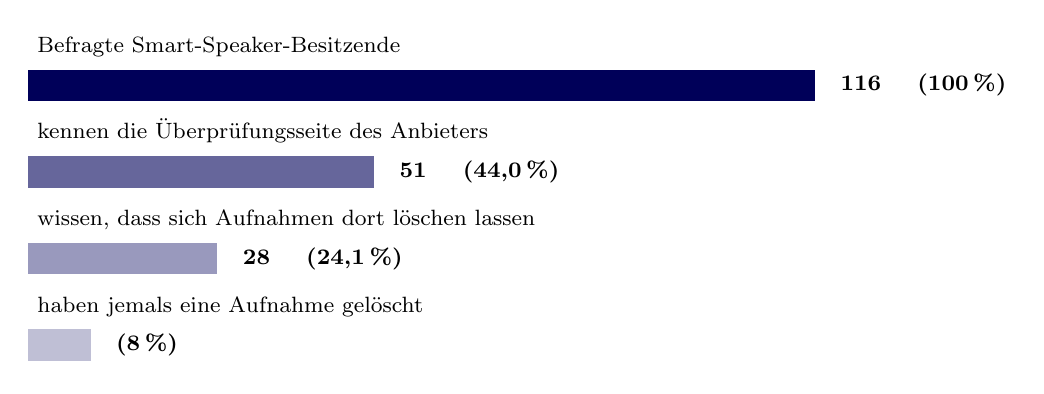
\begin{tikzpicture}[x=1mm,y=1mm]
		% Stufen der Datenkontrolle als Trichter (Balkenbreite = Anteil der Befragten).
		% Zeilenabstand bewusst groesser als die Balkenhoehe, damit jede Beschriftung
		% eindeutig dem Balken darunter zugeordnet werden kann.
		\fill[nakblue]     (0,  0) rectangle (100.0,   4);
		\fill[nakblue!60]  (0,-11) rectangle ( 44.0,  -7);
		\fill[nakblue!40]  (0,-22) rectangle ( 24.1, -18);
		\fill[nakblue!25]  (0,-33) rectangle (  8.0, -29);

		% Beschriftung jeweils unmittelbar oberhalb des zugehoerigen Balkens
		\node[anchor=south west, font=\footnotesize] at (0,  4.4) {Befragte Smart-Speaker-Besitzende};
		\node[anchor=south west, font=\footnotesize] at (0, -6.6) {kennen die Überprüfungsseite des Anbieters};
		\node[anchor=south west, font=\footnotesize] at (0,-17.6) {wissen, dass sich Aufnahmen dort löschen lassen};
		\node[anchor=south west, font=\footnotesize] at (0,-28.6) {haben jemals eine Aufnahme gelöscht};

		% Werte rechts neben den Balken
		\node[anchor=west, font=\footnotesize\bfseries] at (102.0,  2) {116 \quad (100\,\%)};
		\node[anchor=west, font=\footnotesize\bfseries] at ( 46.0, -9) {51 \quad (44,0\,\%)};
		\node[anchor=west, font=\footnotesize\bfseries] at ( 26.1,-20) {28 \quad (24,1\,\%)};
		\node[anchor=west, font=\footnotesize\bfseries] at ( 10.0,-31) {(8\,\%)};
	\end{tikzpicture}
	\caption[Nutzung der Datenschutzfunktionen von Smart Speakern]{Stufen der Datenkontrolle. Eigene Darstellung nach \textcite{malkin2019privacy}.}
	\label{fig:kontrolltrichter}
\end{figure}

Ein dritter Aspekt ist das Drittanbieterökosystem. Von 90.194 analysierten Alexa-Skills legten rund 23,3\,\% derjenigen mit Zugriff auf sensible Daten die betroffenen Datenkategorien nicht vollständig offen. Zudem ist der Backend-Code nach der Zertifizierung veränderbar \cite{lentzsch2021alexa}. Rechtlich erschwert der Audiokanal eine informierte Einwilligung nach der \ac{DSGVO}. Besonders betroffen sind Dritte wie Gäste und Kinder \cite{seymour2023consent}. Dass dies kein theoretisches Risiko ist, belegt ein Verfahren der Federal Trade Commission gegen Amazon von 2023: Sprachaufnahmen von Kindern wurden unbegrenzt gespeichert, Löschanfragen nicht umgesetzt \cite{ftc2023amazon}.

\subsection{IT-Sicherheit}

Die IT-Sicherheit betrifft nicht die reguläre Verarbeitung, sondern die gezielte Kompromittierung durch Dritte. Der strukturelle Schwachpunkt ist der Sprachkanal: weder authentifiziert noch gegen fremde Signale geschützt. Beim DolphinAttack werden Befehle auf Ultraschallträger moduliert und dadurch unhörbar, im Gerät aber dennoch ausgeführt. Der Angriff wurde unter anderem gegen Siri, Google Now, Cortana und Alexa demonstriert \cite{zhang2017dolphin}. Light Commands zeigt, dass sich Mikrofone auf Basis von \ac{MEMS} durch modulierte Laserstrahlung über bis zu 110 Meter und ohne physischen Zugriff ansteuern lassen \cite{sugawara2020light}. Beide unterlaufen das Vertrauensmodell der Geräte, die jede akustisch eintreffende Anweisung als legitim behandeln.

Eine neue Qualität erhält dies durch Assistenten auf Basis großer Sprachmodelle, die Aufgaben eigenständig planen und Werkzeuge einbinden. Verarbeiten sie Inhalte aus nicht vertrauenswürdigen Quellen wie Webseiten oder E-Mails, können dort eingebettete Anweisungen das Systemverhalten übernehmen. Diese als indirekte Prompt Injection bezeichnete Angriffsklasse ist an produktiven Anwendungen nachgewiesen \cite{greshake2023injection}. Das Schadenspotenzial verschiebt sich damit vom einzelnen Befehl zur eigenständigen Handlung eines Systems mit weitreichenden Rechten.

\subsection{Abhängigkeit}
\label{subsec:abhaengigkeit}

Abhängigkeiten wirken auf zwei Ebenen. Technisch-wirtschaftlich liegen die wesentlichen Bestandteile der Infrastruktur bei wenigen global agierenden Anbietern. Die \ac{EU} begegnet dem mit Instrumenten für digitale Souveränität \cite{blancato2024cloud}. Daraus folgen zwei Risiken: Die Ökosysteme sind weitgehend geschlossen, sodass ein Wechsel hohe Kosten verursacht, und die Verfügbarkeit hängt von einer unternehmerischen Entscheidung ab. Das zeigt der im Titel genannte Assistent Cortana, dessen eigenständige Anwendung Microsoft 2023 einstellte \cite{microsoft2023cortana}.

Auf nutzungsbezogener Ebene geht es um die Verlagerung der Urteilsbildung. Zuverlässige Automatisierung führt dazu, dass Menschen ihre Kontrollfunktion vernachlässigen und Systemfehler übersehen. Für die Entscheidungsunterstützung durch \ac{KI} ist dieses Übervertrauen experimentell belegt, ließ sich aber durch eine erzwungene Auseinandersetzung mit dem Vorschlag messbar verringern \cite{bucinca2021trust}. Die Delegation ist damit gestaltbar, aber nicht folgenlos.

\subsection{Ethik}

Ethisch stellt sich die Frage, für wen die Technologie gleich gut funktioniert. Eine Untersuchung von fünf kommerziellen Spracherkennungssystemen ermittelte für afroamerikanische Sprechende eine durchschnittliche Wortfehlerrate von 0,35 gegenüber 0,19 bei weißen Sprechenden \cite{koenecke2020racial}. Das berührt die Argumentation unmittelbar: Wird der Nutzen mit Barrierefreiheit begründet \cite{Esquivel2024}, muss die Erkennung unabhängig von Dialekt, Akzent oder Sprechweise funktionieren. Andernfalls verstärkt die Technologie genau die Zugangsunterschiede, die sie abbauen soll.

Hinzu kommt die Gestaltung: Assistenten werden überwiegend mit weiblich konnotierten Stimmen ausgeliefert und als dienstbare Gegenüber inszeniert, wodurch tradierte Rollenbilder reproduziert werden \cite{sindoni2024feminization}. Da die Interaktion überwiegend befehlend erfolgt und in Haushalten mit Kindern alltäglich ist, wirkt diese Gestaltungsentscheidung gesellschaftlich.

\section{Positionierung (Kettner)}
\label{sec:positionierung}

\subsection{Rückbezug auf Position}

Das vorliegende Papier vertritt die Position, dass der Nutzen intelligenter Assistenten ihre Risiken überwiegt, sofern ihr Einsatz durch klare datenschutzrechtliche und technische Rahmenbedingungen abgesichert wird. Die Befunde widerlegen sie nicht, sie präzisieren sie. Wie bereits Abschnitt~\ref{subsec:cloud} an der Architektur festmacht, folgen die Probleme aus veränderbaren Gestaltungsentscheidungen. Dazu zählen die Auslagerung in die Cloud, unbegrenzte Speicherung als Voreinstellung, ein unzureichend kontrollierter Drittanbietermarkt und ein unauthentifizierter Sprachkanal. Tabelle~\ref{tab:bedingungen} ordnet jedem Befund die Bedingung zu.

\begin{table}[!htb]
	\centering
	\small
	% Linksbuendige Spalten (kein Blocksatz, sonst reissen die schmalen Spalten
	% Loecher) und zusaetzlicher Zeilenabstand, damit die Zellen nicht an den
	% Linien kleben.
	\setlength{\extrarowheight}{2pt}
	\renewcommand{\arraystretch}{1.1}
	\begin{tabularx}{\textwidth}{@{}
			>{\raggedright\arraybackslash}p{2.85cm}
			>{\raggedright\arraybackslash}X
			>{\raggedright\arraybackslash}X @{}}
		\hline
		\textbf{Herausforderung} & \textbf{Empirischer Befund} & \textbf{Abgeleitete Bedingung} \\ \hline
		Datenschutz   & Mehrere hundert Fehlauslösungen              & Lokale Erkennung, Datensparsamkeit \\
		              & 56,0\,\% kennen die Überprüfungsseite nicht  & Sichtbare und überprüfbare Löschung \\
		              & 23,3\,\% der Skills sind intransparent       & Verbindliche Kontrolle der Drittanbieter \\ \hline
		IT-Sicherheit & Einspeisung per Ultraschall und Laser        & Sprecherauthentifizierung \\
		              & Indirekte Prompt Injection                   & Minimale Rechte, Bestätigungspflicht \\ \hline
		Abhängigkeit  & Verarbeitung bei wenigen Anbietern           & Offene Schnittstellen, Datenportabilität \\
		              & Einstellung von Cortana 2023                 & Lokale Rückfallebenen \\
		              & Belegte Übervertrauensbildung                & Bewusste Begrenzung der Delegation \\ \hline
		Ethik         & Wortfehlerrate 0,35 gegenüber 0,19           & Veröffentlichte Prüfung je Sprechergruppe \\
		              & Feminisierte Gestaltung                      & Geschlechtsneutrale Gestaltungsoptionen \\ \hline
	\end{tabularx}
	\caption[Herausforderungen und abgeleitete Bedingungen]{Zuordnung der einzelnen Befunde zu den jeweils daraus abgeleiteten Bedingungen für einen verantwortbaren Einsatz.}
	\label{tab:bedingungen}
\end{table}

Dafür sprechen drei Argumente. Erstens existieren für die zentralen Bedrohungen an der \ac{DSGVO} ausgerichtete Lösungsansätze \cite{HernandezAcosta2022}. Zweitens wirkt regulatorischer Druck, wie die verbindlichen Auflagen im Verfahren gegen Amazon zeigen \cite{ftc2023amazon}. Drittens lässt sich Übervertrauen durch bewusste Interaktionsgestaltung messbar reduzieren \cite{bucinca2021trust}. Dem steht ein bei der Barrierefreiheit nicht substituierbarer Nutzen gegenüber \cite{Esquivel2024}.

Zwei Einwände bleiben offen. Gäste und Kinder werden erfasst, ohne eingewilligt zu haben, und der Audiokanal bietet dafür keine praktikable Lösung \cite{seymour2023consent}. Die Anbieterabhängigkeit ist nur marktseitig und regulatorisch adressierbar \cite{blancato2024cloud}. Wo regelmäßig Dritte erfasst oder besonders schützenswerte Daten verarbeitet werden, etwa in Kinderzimmern oder der Patientenversorgung, ist der Einsatz daher nicht ohne zusätzliche Absicherung vertretbar. Die Position lautet nicht, dass die Risiken gelöst wären, sondern dass sie lösbar sind.

\subsection{Handlungsempfehlungen}

Nutzende sollten die vorhandenen Kontrollmöglichkeiten nutzen: Aufnahmen regelmäßig löschen, das Mikrofon in sensiblen Situationen deaktivieren \cite{malkin2019privacy}, Dritte informieren und Zahlungsfunktionen oder Türschlösser nur mit zusätzlicher Bestätigung koppeln.

Unternehmen sollten den Einsatz als Verarbeitungsvorgang im Sinne der \ac{DSGVO} behandeln und angesichts der Lücken im Drittanbieterökosystem \cite{lentzsch2021alexa} einzelne Anwendungen gezielt freigeben statt pauschal zu öffnen. Für agentische Assistenten gelten zusätzlich minimale Rechte und eine Trennung von Nutzeranweisungen und Fremdinhalten \cite{greshake2023injection}.

Hersteller und Gesetzgeber verantworten die übrigen Bedingungen aus Tabelle~\ref{tab:bedingungen}, insbesondere die Zertifizierung von Drittanbieteranwendungen und die Veröffentlichung der Erkennungsleistung \cite{koenecke2020racial}.

\section{Fazit \& Ausblick (Kettner)}
\label{sec:fazit}

Die Untersuchung bestätigt die eingangs formulierte Position in ihrer bedingten Form: Datenschutz, IT-Sicherheit, Abhängigkeit und Ethik sind keine grundsätzlichen Einwände gegen intelligente Assistenten, sondern die Voraussetzungen eines verantwortbaren Einsatzes. Fehlauslösungen sind messbar \cite{schoenherr2022accidental}, das Wissen der Nutzenden lückenhaft \cite{malkin2019privacy}, der Sprachkanal angreifbar \cite{zhang2017dolphin,sugawara2020light} und die Erkennungsleistung ungleich verteilt \cite{koenecke2020racial}. All diese Befunde gehen auf veränderbare Gestaltungsentscheidungen zurück. Die Abwägung fällt daher zugunsten des Einsatzes aus, jedoch nur unter den benannten Bedingungen.

Deren Bedeutung nimmt künftig zu: Systeme, die Aufgaben eigenständig planen und Werkzeuge einbinden, vergrößern Schadenspotenzial \cite{greshake2023injection} wie Übervertrauensrisiko \cite{bucinca2021trust}. Zugleich erlauben leistungsfähigere Endgeräte eine lokale Verarbeitung, und mit \ac{DSGVO} und \ac{KI}-Verordnung konkretisieren sich die Pflichten der Anbieter \cite{blancato2024cloud}. Ob intelligente Assistenten ihr Potenzial einlösen, entscheidet sich folglich nicht daran, ob die Technologie eingesetzt wird, sondern ob sich datenschutzfreundliche Architekturen gegenüber dem cloudzentrierten Modell durchsetzen.
